%%%%%%%%%%%%%%%%%%%%%%%%%%%%%%%%%%%%%%%%%%%%%%%%%%%%%%%%%%%%%%%%%%%%%%%%%%%%%%%%
%2345678901234567890123456789012345678901234567890123456789012345678901234567890
%        1         2         3         4         5         6         7         8

\documentclass[letterpaper, 10 pt, conference]{ieeeconf}  % Comment this line out if you need a4paper

%\documentclass[a4paper, 10pt, conference]{ieeeconf}      % Use this line for a4 paper

\IEEEoverridecommandlockouts                              % This command is only needed if 
                                                          % you want to use the \thanks command

\overrideIEEEmargins                                      % Needed to meet printer requirements.

%In case you encounter the following error:
%Error 1010 The PDF file may be corrupt (unable to open PDF file) OR
%Error 1000 An error occurred while parsing a contents stream. Unable to analyze the PDF file.
%This is a known problem with pdfLaTeX conversion filter. The file cannot be opened with acrobat reader
%Please use one of the alternatives below to circumvent this error by uncommenting one or the other
%\pdfobjcompresslevel=0
%\pdfminorversion=4

% See the \addtolength command later in the file to balance the column lengths
% on the last page of the document

% The following packages can be found on http:\\www.ctan.org
\usepackage{graphics} % for pdf, bitmapped graphics files
\usepackage{epsfig} % for postscript graphics files
\usepackage{mathptmx} % assumes new font selection scheme installed
\usepackage{times} % assumes new font selection scheme installed
\usepackage{amsmath} % assumes amsmath package installed
\usepackage{amssymb}  % assumes amsmath package installed
\usepackage{mathtools}
\usepackage{relsize}
\usepackage{tikz}
\graphicspath{{./Drawings/}} 

\title{\LARGE \bf
Robustly constrained data-driven control
}


\author{Albert Author$^{1}$ and Bernard D. Researcher$^{2}$% <-this % stops a space
\thanks{*This work was not supported by any organization}% <-this % stops a space
\thanks{$^{1}$Albert Author is with Faculty of Electrical Engineering, Mathematics and Computer Science,
        University of Twente, 7500 AE Enschede, The Netherlands
        {\tt\small albert.author@papercept.net}}%
\thanks{$^{2}$Bernard D. Researcheris with the Department of Electrical Engineering, Wright State University,
        Dayton, OH 45435, USA
        {\tt\small b.d.researcher@ieee.org}}%
}


\begin{document}



\maketitle
\thispagestyle{empty}
\pagestyle{empty}


%%%%%%%%%%%%%%%%%%%%%%%%%%%%%%%%%%%%%%%%%%%%%%%%%%%%%%%%%%%%%%%%%%%%%%%%%%%%%%%%
\begin{abstract}

This is a very skeletal overview.

\end{abstract}


%%%%%%%%%%%%%%%%%%%%%%%%%%%%%%%%%%%%%%%%%%%%%%%%%%%%%%%%%%%%%%%%%%%%%%%%%%%%%%%%
\section{Problem Setup}
Consider a \textit{single-input single-output} system $\mathbb{G}_P$ generating an output signal $y(t) \in \mathbb{R}$ corresponding to the input signal $u(t) \in \mathbb{R}$ for the time $t \in \mathbb{Z}$. Consider the data $\mathbb{D}_{N}=\{u(t),y(t);t\in{1,...,N}\}$ obtained by exciting the system. 
\\
A feedback controller is designed to control the system, using the VRFT methodology. For this, a reference model $\mathbb{M}_P$ is selected. The VRFT methodology designs a feedback controller  $\mathbb{K}_P$, with the goal of making the closed-loop system $\mathbb{K}_P$-$\mathbb{G}_P$ behave similar to the reference model $\mathbb{M}_P$. To this end, the VRFT methodology utilizes the dataset $\mathbb{D}_N$. The desired closed-loop behavior is described by the LTI state-space model $\mathbb{M}_P$ 

	\begin{equation*}
	\begin{matrix}
	x_M(t+1) = A_Mx_M(t) + B_Mg(t)\\
	y_d(t) = C_Mx_M(t)
	\end{matrix}
	\end{equation*}\\    
The VRFT methodology utilized to design the feedback controller $\mathbb{K}_P$ is now explained:
\begin{enumerate}
	\item
	A virtual reference input $g(t)$ is calculated by setting $y_d(t)=y(t)$ obtained from the dataset $\mathbb{D}_N$, by the inverting the model $\mathbb{M}_P$. Let this mapping be defined by $g(t) = \mathbb{M}_P^{\dagger}y(t) $.
	\item
	A feedback controller $\mathbb{K}_P$ described by $A_K(q^{-1})u(t) = B_K(q^{-1})(g(t)-y(t)$ is chosen, where 
	\begin{equation*}
	\begin{matrix}
	A_K(q^{-1}) = 1+\mathlarger{\sum\limits_{i=1}^{n_{a_K}}}a_i^Kq^{-i}\\
	B_K(q^{-1}) = \mathlarger{\sum\limits_{i=1}^{n_{b_K}}}b_i^Kq^{-i}
	\end{matrix}  
	\end{equation*}
	The parameters of the controller $a_i^K$ and $b_i^K$ are calculated by the VRFT methodology, such that the closed loop performance of $\mathbb{K}_P$-$\mathbb{G}_P$ matches open loop performance of  the reference model $\mathbb{M}_P$.
	\item
	This is done by solving the convex optimization problem
	\begin{equation*}
	\begin{aligned}
	& \underset{a_i^K,b_i^K}{\text{min}}
	& & \frac{1}{N}\mathlarger{\sum\limits_{t=1}^N}\mathlarger{\mathlarger{|}}A_K(q^{-1})u(t)-B_K(q^{-1})(\mathbb{M}_P^{\dagger}y(t)-y(t))\mathlarger{\mathlarger{|}}^2 \\
	\end{aligned}
	\end{equation*}
	which minimizes the deviation between the control input calculated by the controller and $u(t)$ that is used to excite the system and obtain $y(t)$.
	\item
	The synthesized controller $\mathbb{K}_P$ is placed before the plant, and the loop is closed. A reference step input is given to evaluate the controller performance.
	\begin{figure}[h]
	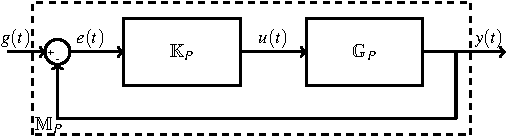
\includegraphics{KpGp.pdf}
	\end{figure}
	
	
	  
\end{enumerate} 

	
                                                              




\begin{thebibliography}{99}

\bibitem{c1} G. O. Young, �Synthetic structure of industrial plastics (Book style with paper title and editor),� 	in Plastics, 2nd ed. vol. 3, J. Peters, Ed.  New York: McGraw-Hill, 1964, pp. 15�64.
\bibitem{c2} W.-K. Chen, Linear Networks and Systems (Book style).	Belmont, CA: Wadsworth, 1993, pp. 123�135.
\bibitem{c3} H. Poor, An Introduction to Signal Detection and Estimation.   New York: Springer-Verlag, 1985, ch. 4.
\bibitem{c4} B. Smith, �An approach to graphs of linear forms (Unpublished work style),� unpublished.
\bibitem{c5} E. H. Miller, �A note on reflector arrays (Periodical style�Accepted for publication),� IEEE Trans. Antennas Propagat., to be publised.
\bibitem{c6} J. Wang, �Fundamentals of erbium-doped fiber amplifiers arrays (Periodical style�Submitted for publication),� IEEE J. Quantum Electron., submitted for publication.
\bibitem{c7} C. J. Kaufman, Rocky Mountain Research Lab., Boulder, CO, private communication, May 1995.
\bibitem{c8} Y. Yorozu, M. Hirano, K. Oka, and Y. Tagawa, �Electron spectroscopy studies on magneto-optical media and plastic substrate interfaces(Translation Journals style),� IEEE Transl. J. Magn.Jpn., vol. 2, Aug. 1987, pp. 740�741 [Dig. 9th Annu. Conf. Magnetics Japan, 1982, p. 301].
\bibitem{c9} M. Young, The Techincal Writers Handbook.  Mill Valley, CA: University Science, 1989.
\bibitem{c10} J. U. Duncombe, �Infrared navigation�Part I: An assessment of feasibility (Periodical style),� IEEE Trans. Electron Devices, vol. ED-11, pp. 34�39, Jan. 1959.
\bibitem{c11} S. Chen, B. Mulgrew, and P. M. Grant, �A clustering technique for digital communications channel equalization using radial basis function networks,� IEEE Trans. Neural Networks, vol. 4, pp. 570�578, July 1993.
\bibitem{c12} R. W. Lucky, �Automatic equalization for digital communication,� Bell Syst. Tech. J., vol. 44, no. 4, pp. 547�588, Apr. 1965.
\bibitem{c13} S. P. Bingulac, �On the compatibility of adaptive controllers (Published Conference Proceedings style),� in Proc. 4th Annu. Allerton Conf. Circuits and Systems Theory, New York, 1994, pp. 8�16.
\bibitem{c14} G. R. Faulhaber, �Design of service systems with priority reservation,� in Conf. Rec. 1995 IEEE Int. Conf. Communications, pp. 3�8.
\bibitem{c15} W. D. Doyle, �Magnetization reversal in films with biaxial anisotropy,� in 1987 Proc. INTERMAG Conf., pp. 2.2-1�2.2-6.
\bibitem{c16} G. W. Juette and L. E. Zeffanella, �Radio noise currents n short sections on bundle conductors (Presented Conference Paper style),� presented at the IEEE Summer power Meeting, Dallas, TX, June 22�27, 1990, Paper 90 SM 690-0 PWRS.
\bibitem{c17} J. G. Kreifeldt, �An analysis of surface-detected EMG as an amplitude-modulated noise,� presented at the 1989 Int. Conf. Medicine and Biological Engineering, Chicago, IL.
\bibitem{c18} J. Williams, �Narrow-band analyzer (Thesis or Dissertation style),� Ph.D. dissertation, Dept. Elect. Eng., Harvard Univ., Cambridge, MA, 1993. 
\bibitem{c19} N. Kawasaki, �Parametric study of thermal and chemical nonequilibrium nozzle flow,� M.S. thesis, Dept. Electron. Eng., Osaka Univ., Osaka, Japan, 1993.
\bibitem{c20} J. P. Wilkinson, �Nonlinear resonant circuit devices (Patent style),� U.S. Patent 3 624 12, July 16, 1990. 






\end{thebibliography}




\end{document}
